A controller hardware in the loop (CHIL) simulation was set up to validate the algorithm in a real-time environment. 
The block layout of the CHIL simulation is shown in Fig. \ref{fig:RT_block}. The power system shown in Fig. \ref{fig:simulation_grid}, is simulated in real time in a digital real-time simulator (DRTS) with a time step of 50 ${\mu}s$. This system is modeled for detailed electromagnetic transient simulation unlike the phasor simulation model used in the offline simulation. The A* based ESM algorithm is implemented in Python 2.7 on a windows machine. The specifications of the machine are given in Table \ref{tab:PC}. The communication link between the DRTS and windows machine was established using TCP/IP. The DRTS sent the windows machine running the ESM the current PV generation ($P_{PV}(t)$), the current load ($P_load(t)$) and the current energy storage state of charge ($ES_{SOC}(t)$). The RTP, Load and PV prediction profiles are fed to the ESM by a pregenerated MATLAB formatted data (MAT) file. The current RTP is also provided by the MAT file. After receiving the current status and predicted profiles the ESM determines the power the ES should provide for the current time period ($P_{ES}(t)$) and sends it back to the DRTS. The actual CHIL setup is shown in Fig. \ref{fig:LAB_REAL}.

\begin{table}[htb]
\caption{Windows machine specification}
\label{tab:PC}
\centering
\begin{tabular}{|l|l|}
\hline
Operating system & Windows 10 Home 64-bit      \\ \hline
Processor        & Intel(R) Core(TM) i5-7300HQ \\ \hline
Memory           & 8192 MB RAM                 \\ \hline
\end{tabular}
\end{table}

\begin{figure}[!ht]
    \centering
    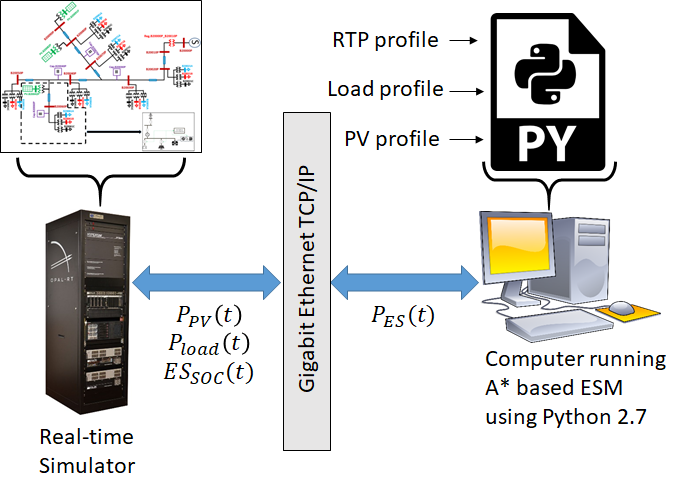
\includegraphics[width = \linewidth]{figs/A8/RT_block.png}
    \caption{Block layout of the CHIL setup}
    \label{fig:RT_block}
\end{figure}

\begin{figure}[!ht]
    \centering
    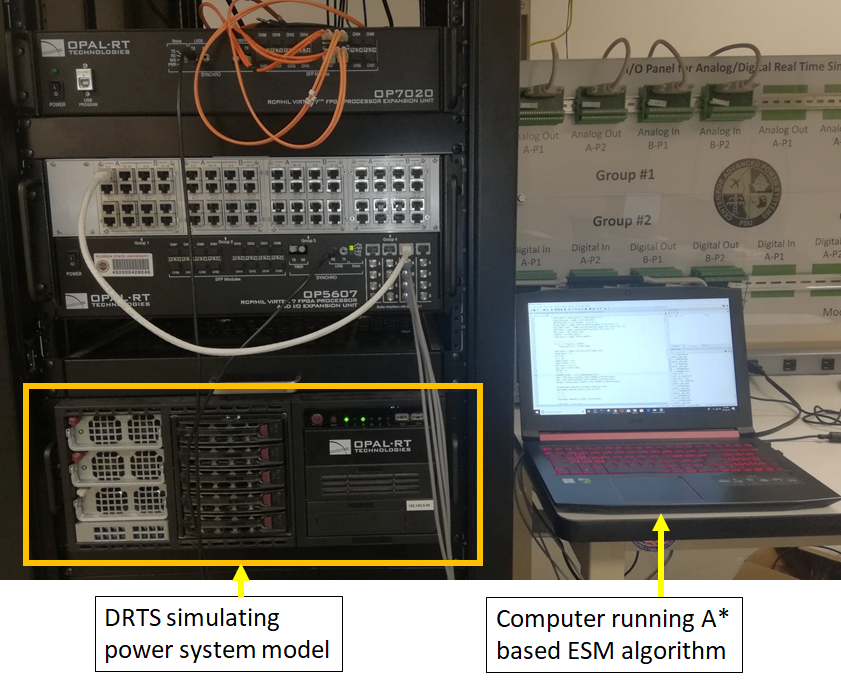
\includegraphics[width = \linewidth]{figs/A8/LAB_REAL.png}
    \caption{Actual CHIL setup}
    \label{fig:LAB_REAL}
\end{figure}

For the CHIL simulation, the ESM algorithm was set up according to the setup described in Section \ref{OFF}. The simulation was run for 50 hours (200 time steps) in real-time. Fig. \ref{fig:RT_TESTING} shows the real-time and the offline simulation results for the 50 hour run. It can be seen that the real-time simulation result shown by the dotted lines follows the off-line simulation result shown by the solid line. The results are similar to the first two days of Fig. \ref{fig:SBMPO_COMP_10_12} as expected. The comparison of the real-time and offline cost savings of the algorithm is shown in table \ref{tab:rt_cost}. It can be seen from the table that the real-time cost savings is comparable to the offline results.

\begin{figure}[!ht]
    \centering
    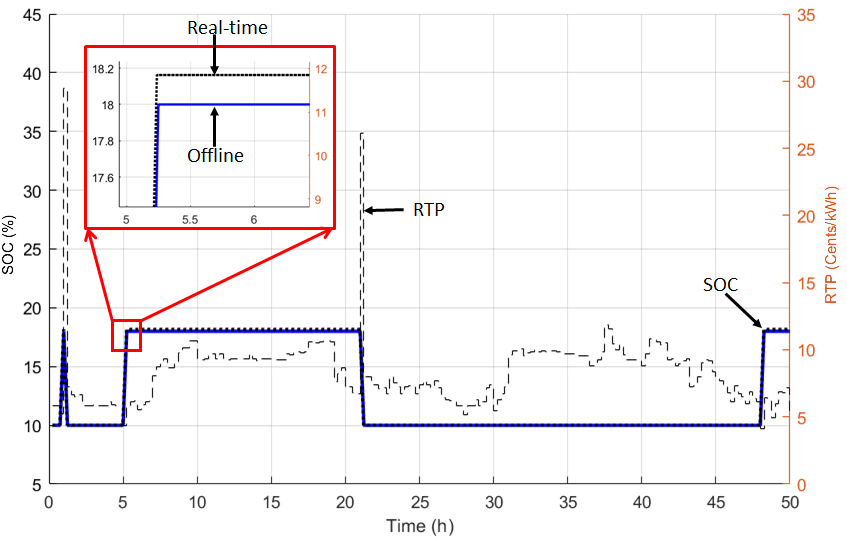
\includegraphics[width = \linewidth]{figs/A8/RT_TESTING.png}
    \caption{Real-time vs offline result (50  hours)}
    \label{fig:RT_TESTING}
\end{figure}

\begin{table}[htb]
\centering
\caption{Real-time simulation cost (48 hours)}
\label{tab:rt_cost}
\begin{tabular}{l|l|l|l|}
\cline{2-4}
                                          & Real-time & Offline & Difference \\ \hline
\multicolumn{1}{|l|}{Case1}               & \$1,662   & \$1,579 & 4.99\%     \\ \hline
\multicolumn{1}{|l|}{Cas2}                & \$1,713   & \$1,628 & 4.96\%     \\ \hline
\multicolumn{1}{|l|}{A* Case}             & \$1,345   & \$1,286 & 4.39\%     \\ \hline
\multicolumn{1}{|l|}{A* savings (Case 1)} & 19.07\%   & 18.56\% & 0.52\%     \\ \hline
\multicolumn{1}{|l|}{A* savings (Case 2)} & 21.48\%   & 21.01\% & 0.48\%     \\ \hline
\end{tabular}
\end{table}